\chapter[Evaluation]{Evaluation}

In this chapter, the NVM Middleware and the Q-Learning Model.

\section{Experimental Setup}

\subsection{Platform}

\begin{table}[ht]
    \centering
    \caption{Experimental Platform Specifications}
    \label{table:platform_specifications}
    \begin{tabular}{|l|l|}
      \hline
      Processor & Intel\,\textsuperscript{\tiny\textregistered} Xeon\,\textsuperscript{\tiny\textregistered} Gold 6252   \\\hline
      Sockets & 2 \\\hline
      Cores per socket & 24  \\\hline
      Threads per core & 2 \\\hline
      Numa nodes & 2 \\\hline
      CPU Frequency & 2.7 GHz (3.7 GHz Turbo frequency) \\\hline
      L1d cache & 1.5 MiB  \\\hline
      L1i cache & 1.5 MiB  \\\hline
      L2 Cache & 48 MiB  \\\hline
      L3 Cache & 71.5 MiB  \\\hline
      DRAM & 16 GB DDR4 DIMM x 6 per socket  \\\hline
      Persistent Memory & 128 GB Optane PMM x 6 per socket  \\\hline
      Operating System & Ubuntu 20.04.4 LTS (Focal Fossa)  \\\hline
      \hline
    \end{tabular}
\end{table}

The experimental platform utilized in this study is detailed in Table \ref{table:platform_specifications}. It features an Intel,\textsuperscript{\tiny\textregistered} Xeon,\textsuperscript{\tiny\textregistered} Gold 6252 processor with 2 sockets, each hosting 24 cores and 2 threads per core, totaling 2 NUMA nodes. Each socket is equipped with three memory channels, housing 16 GB DDR4 DIMMs and 128 GB Optane PMMs. In aggregate, the system comprises 192 GB of DRAM and 1.5 TB of Optane persistent memory. To mitigate the NUMA effect, one socket is designated for running the NVM Middleware threads, while the other handles the interactive and batch applications, as described in Section 3.4.3.

\subsection{Optane DC PMem Configuration}
As outlined earlier, this thesis concentrates on exploring the persistent capabilities of Optane DC PMem. Consequently, Optane DC PMem is employed in the App Direct Mode throughout our experiments. To facilitate the utilization of persistent memory, we expose it via an xfs filesystem configured in dax mode, thereby bypassing the page cache. Additionally, we enhance memory management and performance by configuring the persistent memory with huge pages (2MiB) \cite{Speeding28:online}. Lastly, we deploy a PMEMKV database with a capacity of 600GB, configured with its persistent concurrent engine.

\subsection{Workload Generators}

To execute the interactive and batch applications described in Section 3.4.3, we implement two workload generators.

\textbf{YCSB}. 

For the interactive application, we utilized traces collected from Azure Functions. The dataset, available in \cite{GitHubAz35:online}, offers a comprehensive record of Azure Function blob accesses spanning November to December 2020. Our focus was on requests occurring between November 1 and November 5, particularly those with small data access sizes (less than 1 KB), which are indicative of interactive applications.

For the batch application, we gathered traces from Wukong, a serverless parallel computing framework \cite{carver2020wukong}. Traces were obtained by executing a Single Value Decomposition for a 128x128 matrix on Wukon and capturing the I/O requests generated by the framework. These collected traces represent the behavior of a throughput-oriented serverless data-analytics application.

To further amplify the concurrency of requests directed to the NVM Middleware, we accelerated the pace of the traces by a factor of 5 compared to their original timing.

\section{Efficiency of the Workload-Aware Concurrency Control Mechanism}

Utilizing the environment delineated in Section 3.4.3, we assess the efficacy of the workload-aware concurrency control mechanism integrated into the NVM Middleware against a baseline scenario lacking any concurrency control. In the baseline scenario, the concurrency cotrol mechanism is disabled, allowing a maximum of 200 concurrent data accesses on Optane DC PMem. For this examination, we deactivate the reinforcement learning agent and system monitoring, focusing primarily on the 99th percentile latency and throughput observed by the client applications.

In this experiment, we execute YCSB and SVD Trace Replay concurrently. YCSB is configured with a zipfian request distribution, 128B data access size, and a 50/50 read-to-write ratio. Additionally, each application is run with 100 client threads.

The baseline scenario is executed without any concurrency control, alongside 42 additional tests where various combinations of interactive and batch threads within the NVM Middleware are explored. In each run, a combination of $I$ (interactive) and $B$ (batch) threads is defined and held constant throughout the run. Subsequently, the 99th percentile latency observed by the YCSB requests is recorded, and the overall throughput reported by SVD Trace Replay is captured. The results are presented in Figure \ref{fig:middleware_eval}.

\begin{figure}[ht]
  \centering
  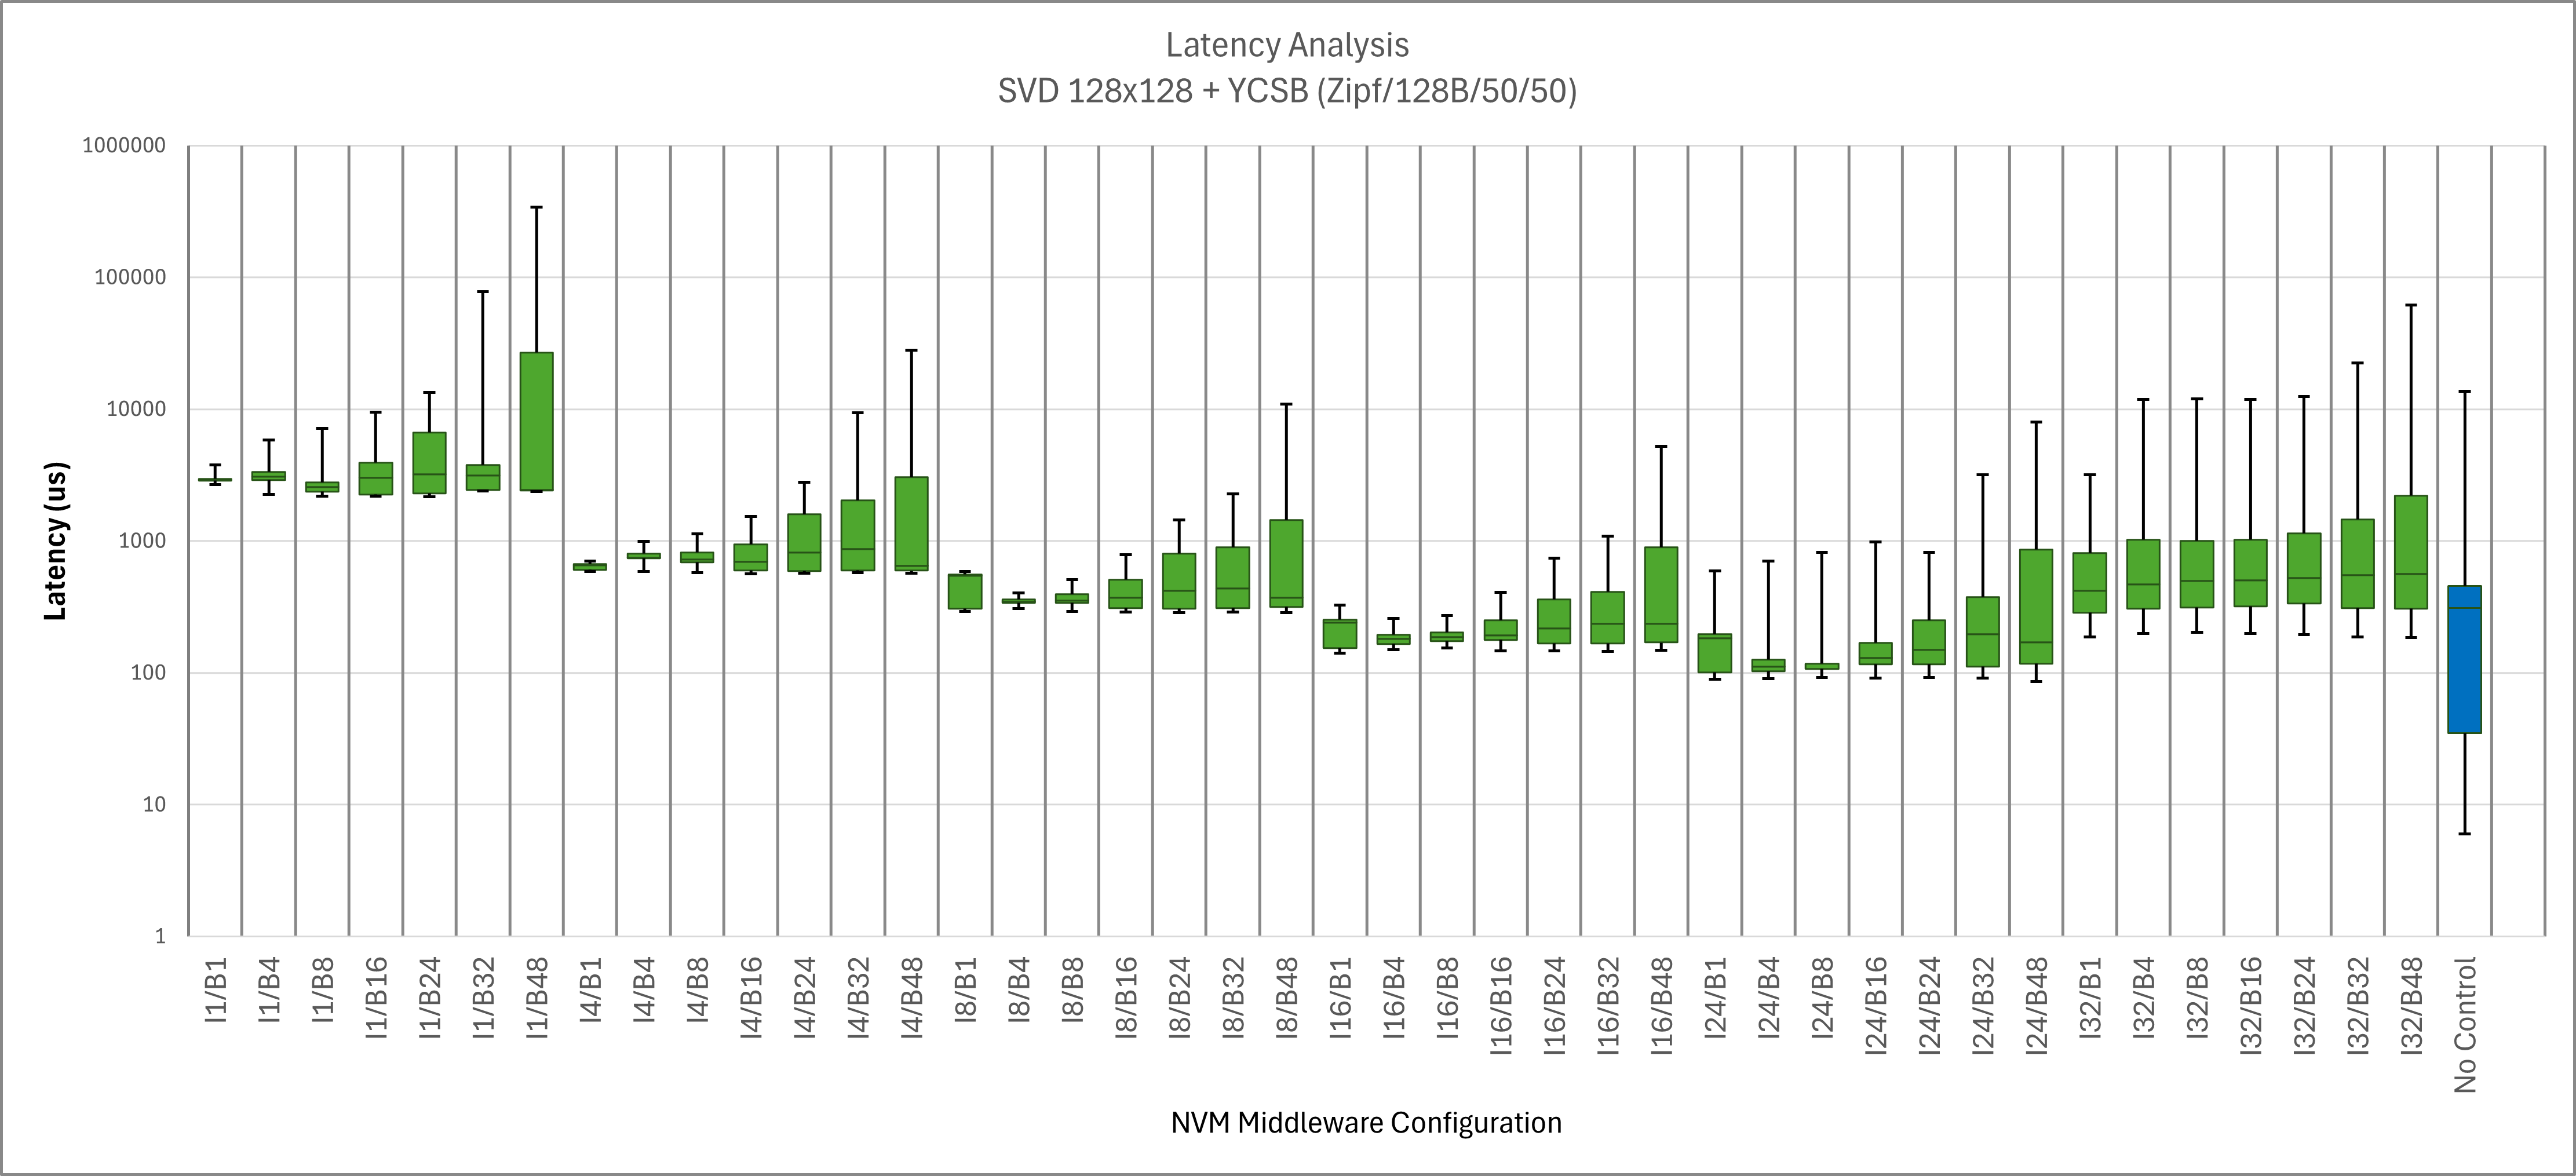
\includegraphics[width=\textwidth,height=\textheight,keepaspectratio,angle=0]{images/middleware-latency.png}
  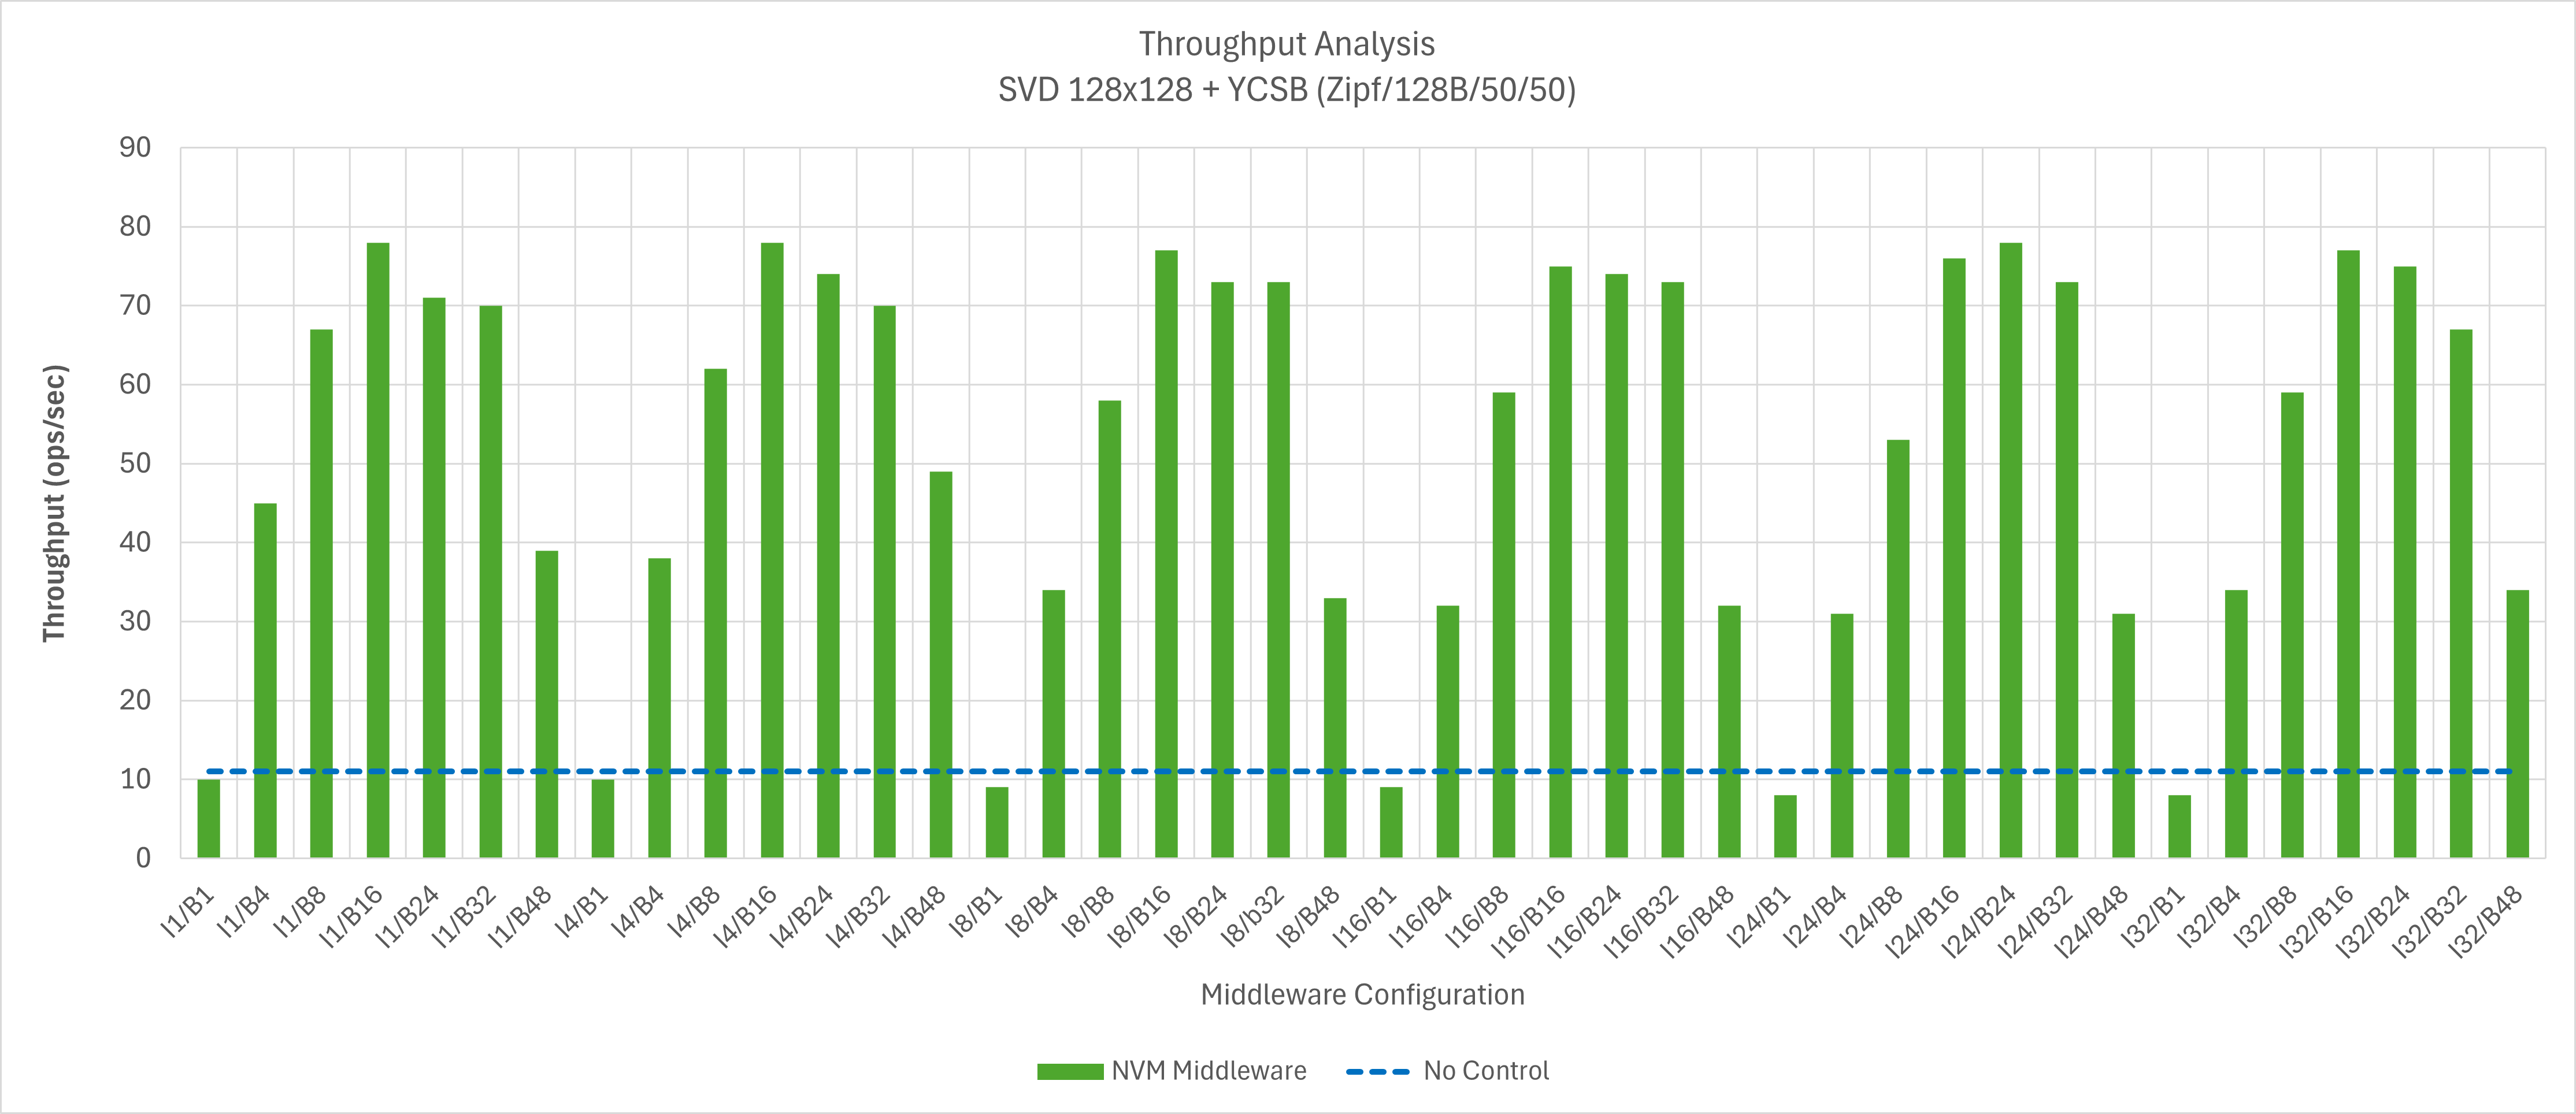
\includegraphics[width=\textwidth,height=\textheight,keepaspectratio,angle=0]{images/middleware-tp.png}
  \caption{Middleware Evaluation}
  \label{fig:middleware_eval}
\end{figure}

Our observations reveal that in most scenarios, both workloads derive substantial benefits from the concurrency control implemented by the NVM Middleware. Relative to the baseline, the NVM Middleware demonstrates the potential to enhance the 99th latency and throughput by up to 98\% and 86\%, respectively. Furthermore, the baseline shows that the 99th latency can vary by X\% orders of magniture, while the NVM Middleware exhibits a more controlled and predictable access latencies. Notably, the figure illustrates that the performance of applications is generally improved across most thread combinations. However, improper configuration of threads within the NVM Middleware, either too few or too many, leads to performance degradation surpassing that of the baseline. This underscores the importance for operators to meticulously select the optimal combination of threads, as an incorrect choice can yield inferior results compared to operating without any concurrency control.

A significant query stemming from these findings pertains to how an operator can determine the optimal thread combination. We observe that combining 16 interactive threads with fewer than 8 batch threads yields superior latency but fails to achieve peak throughput performance. Conversely, any combination with more than 16 batchs threads achieves peak throughput but incurs elevated access latencies. To address this dilemma, the ideal approach involves selecting the combination of interactive and batch threads that satisfies both latency and throughput SLA metrics, a topic further elaborated upon in the subsequent section.

\section{Meeting SLA performance using RL}
We now provide an evaluation of the RL-driven policies to balance the number of interactive and batch threads to meet latency and throughput SLAs. In this experiment, the goal of the NVM MIddleware is to meet pre-defined SLA objectives under changing workloads. To do this, we build four different workload phases by modifying the data access size, and read/write ratio, and client threads of the interactive and batch Trace applications described in Section 6.1.3. For each phase, we train the RL agent to learn the optimal combination of interactive and batch threads that meet pre-defined latency and throughput SLAs, while maximizing performance. Finally, we measure the agent's ability to predict and adapt to workload changes in an unknown environment where the phases are randomly alternated. 

We use the following workloads to train and test the RL agent:

Phase 1. We change the interactive traces to use a data access size of 50B, a read-to-write ratio of 80-20, and 200 concurrent client threads. We change the batch traces to use a data access size of 8k, read-to-write ratio of 50-50, and 200 concurrent client threads. 

Phase 2. We change the interactive traces to use a data access size of 50B, a read-to-write ratio of 80-20, and 150 concurrent client threads. We change the batch traces to use a data access size of 8k, read-to-write ratio of 50-50, and 320 concurrent client threads.  

Phase 3. We change the interactive traces to use a data access size of 50B, a read-to-write ratio of 80-20, and 400 concurrent client threads. We change the batch traces to use a data access size of 4k, pure read, and 200 concurrent client threads.  

Phase 4. We change the interactive traces to use a data access size of 500B, a read-to-write ratio of 10-90, and 200 concurrent client threads. We change the batch traces to use a data access size of 4k, pure read, and 200 concurrent client threads. 

\subsection{Training the RL agent}

We start the learning process by tuning the hyper-parameters of the 9 linear regression models used by the RL agent. To do this, we generate a dataset of transitions in the environment by running a non-optimal random agent on the environment. We run 150 episodes of each phase and let the random agent take random actions on the environment, logging the transitions and the rewards obtained by each transition. Since each linear regression model is supposed to approximate the value function of an action, we build 9 different sub-datasets, where each dataset contains only the transitions observed by taking a specific action. We use each sub-dataset to tune the hyperparameters of a linear regression model that represents action a, choosing from the parameters (Table \ref{table:hyperparameter_tuning}) that best fits the data. The resulting hyperparameters per model are described in Table \ref{table:per_model_parameters}.

\begin{table}[ht]
  \centering
  \caption{Hyper-parameter Tuning}
  \label{table:hyperparameter_tuning}
  % Tabular environment goes AFTER the caption!
  % \begin{adjustbox}{width=1\textwidth}
  \begin{tabular}{|l|l|l|}
    % after \\: \hline or \cline{col1-col2} \cline{col3-col4} ...
    \hline
    \thead{Type} & \thead{Parameter} & \thead{Values} \\
    \hline
    Preprocessing & Degree & 1,2,3 \\\hline
    Regression & alpha & 0.1, 0.01, 0.001, 0.0001 \\\hline
    Regression & penalty & l1, l2, elasticnet \\\hline
    Regression & loss & squared, huber, epsilon\_insensitive \\\hline
    Regression & learning rate & constant, optimal, invscaling \\\hline
    Regression & max\_iterations & 100, 1000, 10000, 100000 \\
    \hline
  \end{tabular}
% \end{adjustbox}
\end{table}

\begin{table}[ht]
  \centering
  \caption{Per-Model tuned hyper-parameters}
  \label{table:per_model_parameters}
  % Tabular environment goes AFTER the caption!
  \begin{adjustbox}{width=1\textwidth}
  \begin{tabular}{|l|l|l|}
    % after \\: \hline or \cline{col1-col2} \cline{col3-col4} ...
    \hline
    \thead{Model} & \thead{Action} & \thead{Parameters} \\
    \hline
    Model\_1 & 1 & learning\_rate: invscaling, loss: squared\_loss, alpha: 0.001, max\_iter: 10000, penalty: l2 \\\hline
    Model\_2 & 2 & learning\_rate: invscaling, loss: squared\_loss, alpha: 0.0001, max\_iter: 1000, penalty: l2 \\\hline
    Model\_3 & 3 & learning\_rate: invscaling, loss: squared\_loss, alpha: 0.001, max\_iter: 1000, penalty: elasticnet \\\hline
    Model\_4 & 4 & learning\_rate: invscaling, loss: squared\_loss, alpha: 0.0001, max\_iter: 10000, penalty: l1 \\\hline
    Model\_5 & 5 & learning\_rate: invscaling, loss: squared\_loss, alpha: 0.01, max\_iter: 100, penalty: elasticnet \\\hline
    Model\_6 & 6 & learning\_rate: invscaling, loss: squared\_loss, alpha:  0.001, max\_iter: 10000, penalty: l2 \\\hline
    Model\_7 & 7 & learning\_rate: invscaling, loss: squared\_loss, alpha: 0.01, max\_iter: 1000, penalty: elasticnet \\\hline
    Model\_8 & 8 & learning\_rate: invscaling, loss: squared\_loss, alpha: 0.001, max\_iter: 100, penalty: l1 \\\hline
    Model\_9 & 9 & learning\_rate: invscaling, loss: squared\_loss, alpha: 0.0001, max\_iter: 100, penalty: elasticnet \\
    \hline
  \end{tabular}
\end{adjustbox}
\end{table}

Using the tuned linear regressoin models, we proceed to run the Q-learning algorithm for each phase using the parameters outlined in Table \ref{table:rl_training_parameters}. We address the exploration-exploitation dilemma by starting with epsilon 1 and decaying it after each episode. This causes the agent to fully explore the state space at the beginning of the training and exploit this knowledge towards the end. We observe that different phases require different training episodes to converge to an optimal pattern. We believe this is expected given that the dataset use to pre-train the models was generated with a non-optimal policy. The random agent might have been stuck in a non-optimal loop of actions and might have not generated good training samples. Therefore, the agent requires additional training to fully capture the characteristics of these phases.

\begin{table}[ht]
  \centering
  \caption{RL Training Parameters}
  \label{table:rl_training_parameters}
  % Tabular environment goes AFTER the caption!
  % \begin{adjustbox}{width=1\textwidth}
  \begin{tabular}{|l|l|}
    % after \\: \hline or \cline{col1-col2} \cline{col3-col4} ...
    \hline
    \thead{Parameter} & \thead{Value} \\
    \hline
    episodes & Phases 1\-2: 700, Phases 3\-4: 1,000 \\\hline
    Per-episode steps & 200 \\\hline
    gamma & 0.95 \\\hline
    learning rate & 0.7 \\\hline
    epsilon & 0.9 \\\hline
    epsilon\_decay & 0.1 \\
    \hline
  \end{tabular}
% \end{adjustbox}
\end{table}

\subsection{Pattern Convergence}
For earch phase, we analyze the last three episodes to determine the combination of threads to which the agent converges. We choose the last three episodes because at that point the agent is exploiting the knowledge obtained from previous episodes.

\subsubsection*{Phase 1}
We observe that the RL agent converges to 10 interactive threads and 10 batch threads. The results are showing in figure X.

\subsubsection*{Phase 2}
We observe that the RL agent converges to 10 interactive threads and 10 batch threads. The results are showing in figure X.

\subsubsection*{Phase 3}
We observe that the RL agent converges to 10 interactive threads and 10 batch threads. The results are showing in figure X.

\subsubsection*{Phase 4}
We observe that the RL agent converges to 10 interactive threads and 10 batch threads. The results are showing in figure X.

\section{Evaluation on long-running test}
We now evaluate our trained model in a scenario where we randomly alternate the phases. We run the agent against the enviroment and run 4000 steps of the simulation, alternating a random workload every 200 steps. We compare the agent's performance against a baseline were we alternate the phases but we fixe the combination of threads in the NVM MIddleware to 15 interactive and 15 batch threads. Figure X shows the results. Table X presents a reward analysis.
